\documentclass[../thesis.tex]{subfiles}

\providecommand{\zcut}{z_\mathrm{{cut}}}
\providecommand{\LIPS}{\mathrm{LIPS}}
\providecommand{\cusp}{\mathrm{cusp}}
\providecommand{\mMDT}{\mathrm{mMDT}}
\providecommand{\Li}{\mathrm{Li}}

\providecommand{\arctanh}{\mathrm{arctanh}}

\providecommand{\cM}{\mathcal{M}}
\providecommand{\cL}{\mathcal{L}}
\providecommand{\cO}{\mathcal{O}}


\setlength{\parskip}{0pt}
%%
%% End Preamble
%%
%% The fun begins:
\begin{document}
	Recall that the goal of our all-orders calculation is to derive an expression which systematically accounts for logarithmic contributions at every order in $\alpha_s$ and with which, if one has sufficient patience and mathematical skill, one could compute the heavy hemisphere mass to arbitrary accuracy in the $\rho \sim \zcut \ll 1$ limit. In this chapter, we will see how this is done.

	As we have repeated several times by now,\footnote{Because it bears repeating!} QCD is a scale-invariant theory. However, when we compute something like the groomed heavy hemisphere mass distribution, we impose scale onto the system (such as the hemisphere mass or the groomer energy cut). In QCD, whenever multiple scales appear, say $\Lambda_h$ and $\Lambda_\ell$, high-order corrections to observables appear with the form \cite{becher_introduction_2015-1}
	\begin{equation}
		\alpha_s^n \log^{n}\frac{\Lambda_h}{\Lambda_\ell}.
	\end{equation}
	These logarithms can grow quite large if the scales are far apart, which enhances the size of these contributions \cite{schwartz_quantum_2014}. Moreover, since these contributions occur at every order in $\alpha_s$, they can be difficult to take care of. This leaves us in a quandary --- how do we handle large corrections which are, for all intents an purposes, out of computational reach?

	The key to an all-orders calculation of the distribution is to keep track of these logarithmic corrections in a systematic way, move them around, and put them back together into a scale-invariant function. This is the process of \textbf{resummation}, which we are about to undertake.

\section{Resummation}\label{all-sec:resummation}
	The first step towards resummation in SCET is to derive a factorization formula \cite{becher_introduction_2015-1}, as we have already done in Eq.~\ref{factor-eq:factorization formula}. Splitting the cross section into terms, each of which depends only on a single scale, enables resummation of each term \cite{frye_factorization_2016}.

	It will be helpful to work in Laplace space, which for a function $f(t)$ is achieved by the transformation \cite{boas_mathematical_2006}
	\begin{equation}
		\cL\qty{f}(s) = \int_0^\infty f(t) e^{-st}\,dt.
	\end{equation}
	For notational simplicity, instead of writing $\cL\qty{f}(s)$ everywhere, we will simply write $f(s)$. That is, whenever a function is written in terms of Laplace variables, we will assume that it is the Laplace-transformed function, and vice versa.

	Under Laplace transformation, convolution becomes multiplication, so under the transformation $\rho \to \nu$, the factorization formula becomes
	\begin{equation}\label{all-eq:factorization formula laplace}
	\begin{aligned}
		\frac{d^2\sigma}{d\nu_1 d\nu_2} = 2 H(Q^2) \times R(\nu_1, \nu_2, \zcut) \times S_R(\nu_1 - \zcut) &\times J_q(\nu_1) \times J_g(\nu_1, \zcut) \\
		&\qquad\times J_{\bar q}(\nu_2) \times S_C(\sqrt{\nu_2 \zcut}).
	\end{aligned}
	\end{equation}
	The multiplicative factorization in Laplace space allows us to resum each term individually, without worrying about cross-talk between terms \cite{frye_factorization_2016}. Before moving on, with this calculation, let us study how our resummation strategy will work.

\subsection{Strategy}
	Let us consider the simple example of a cross section which factorizes into the product of two terms:
	\begin{equation}
		\sigma = F_1 F_2.
	\end{equation}
	Suppose we are working in $d = 4 - 2\epsilon$ dimensions and have introduced a mass scale $\mu$ to compensate for dimensionality changes. We call $\mu$ the \textbf{renormalization scale}. Since $\mu$ is an arbitrary scale introduced to regulate the calculation, the physical quantity $\sigma$ must be independent of $\mu$ at the end of the day:
	\begin{equation}\label{all-eq:partial sigma mu zero}
		\frac{\partial \sigma}{\partial \mu} = 0.
	\end{equation}
	In 4 dimensions, this would be true of $F_1$ and $F_2$ as well. But in our dimensional regularization scheme, away from 4 dimensions, these functions \textit{do} have $\mu$-dependence. Their departure from $\mu$-independence is described by a quantity called the \textbf{anomalous dimension}, so-called because the behavior away from 4 dimensions is anomalous in this sense. If $F_1$ has an anomalous dimension $\gamma_1$ and $F_2$ has an anomalous dimension $\gamma_2$, then it is a general fact of quantum field theory that \cite{schwartz_quantum_2014}
	\begin{align}\label{all-eq:toy RGE}
		\frac{\partial F_1}{\partial \log \mu} &= \gamma_1 F_1 & \frac{\partial F_2}{\partial \log \mu} &= \gamma_2 F_2.
	\end{align}
	In fact, many authors (such as the author of Ref.~\cite{schwartz_quantum_2014}) \textit{define} the anomalous dimension this way. Now notice that this yields, by the product rule,
	\begin{equation}
		\frac{\partial \sigma}{\partial \log \mu} = (\gamma_1 + \gamma_2) F_1 F_2.
	\end{equation}
	In order to enforce Eq.~\ref{all-eq:partial sigma mu zero}, we demand that
	\begin{equation}\label{all-eq:toy anomalous dimension sum}
		\gamma_1 + \gamma_2 = 0.
	\end{equation}
	This provides constraints on our calculations as well as a strong consistency check --- if we have calculated $F_1$ and $F_2$ and find that Eq.~\ref{all-eq:toy anomalous dimension sum} is unsatisfied, then we know a mistake has been made. On the other hand, it means that if we compute the anomalous dimension of $F_1$, then we do not need to compute the anomalous dimension of $F_2$.

	Equations \ref{all-eq:partial sigma mu zero} and \ref{all-eq:toy RGE} are known as \textbf{renormalization group equations}.\footnote{The renormalization group refers to the symmetry of physical quantities under changes in the techniques used to calculate them. Technically, we are working with the \textbf{continuum renormalization group}, which formalizes the independence of observable quantities on $\mu$ in dimensional regularization \cite{schwartz_quantum_2014}.} The overall strategy to resum large logarithms in the cross section $\sigma$ is to solve the renormalization group equation for each function $F_1$ and $F_2$. As long as $\sigma$ factorizes as claimed and Eq.~\ref{all-eq:toy anomalous dimension sum} is satisfied, then this results in an all-orders calculation of $\sigma$.

	Thus, we have a general two-step strategy for resumming a function $F$ (such as $F_1$ or $F_2$ in the example above):
	\begin{enumerate}
		\item Compute the anomalous dimension $\gamma$ of $F$. This is done by computing $F$ to some desired order in $\alpha_s$ and pulling out the appropriate terms. 

		\item Solve the renormalization group equation
		\begin{equation}\label{all-eq:general RGE}
			\frac{\partial F}{\partial \log \mu} = \gamma F = \qty(\Gamma_F(\alpha_s) \log\frac{\mu^2}{\mu_1^2} + \gamma_F(\alpha_s))F.
		\end{equation}
	\end{enumerate}
	These steps are explained in more detail below.

\subsection{Anomalous dimension}

	In order to solve the renormalization group equation, we need to know more about the anomalous dimensions. In general, for a function $F$, the anomalous dimension $\gamma$ can be written as \cite{frye_factorization_2016}
	\begin{equation}\label{all-eq:general anomalous dimension}
		\gamma = \Gamma_F(\alpha_s) \log\frac{\mu^2}{\mu_1^2} + \gamma_F(\alpha_s).
	\end{equation}
	Here, $\mu_1$ is the remainder of the scale appearing with $\mu$ in the logarithm. We call $\Gamma_F(\alpha_s)$ the \textbf{cusp anomalous dimension}, and $\gamma_F(\alpha_s)$ is the \textbf{non-cusp anomalous dimension}. The cusp anomalous dimension is universal up to normalization and can be written as a series in $\alpha_s$:
	\begin{equation}\label{all-eq:general cusp anomalous dimension}
		\Gamma_F(\alpha_s) = d_F \Gamma_\cusp(\alpha_s) = d_F \sum_{n = 0}^\infty \Gamma_n \qty(\frac{\alpha_s}{4\pi})^{n + 1}.
	\end{equation}
	The coefficients $\Gamma_n$ can be pulled from the literature. The relevant terms for our purposes are \cite{frye_factorization_2016}
	\begin{equation}\label{all-eq:Gamma values}
	\begin{aligned}
		\Gamma_0 &= 4 \\
		\Gamma_1 &= 4C_A \qty(\frac{67}{9} - \frac{\pi^2}{3}) - \frac{80}{9}T_R n_f,
	\end{aligned}
	\end{equation}
	where $C_A = 3$ and $T_R = 1/2$ are color factors from QCD and $n_f$ is the number of quarks with energy less than that being considered.

	The real work comes from computing the non-cusp anomalous dimension
	\begin{equation}\label{all-eq:general non-cusp anomalous dimension}
		\gamma_F(\alpha_s) = \sum_{n = 0}^\infty \gamma_n \qty(\frac{\alpha_s}{4\pi})^{n + 1}.
	\end{equation}
	An example calculation will be performed in Sec.~\ref{all-sec:soft function calculation}. This entails computing the function of interest to the desired accuracy, then peeling off the non-logarithmic contributions to the anomalous dimension. The anomalous dimension can be determined either through inspection, by simply taking the coefficient of $2/\epsilon$ (the factor of $2$ comes from the fact that we are working in $d = 4 - 2\epsilon$ dimensions; if we were working in $4 - \epsilon$ dimensions, then we would seek the coefficient of $1/\epsilon$), or by computing the appropriate derivative per the renormalization group equation.

\subsection{Solving the renormalization group equation}\label{all-sec:solving RGE}
	To solve the renormalization group equation, Eq.~\ref{all-eq:general RGE}, it is convenient to rewrite the differential equation not in terms of $\mu$, but in terms of $\alpha_s$. This is done through the QCD $\beta$-function, which describes how $\alpha_s$ depends on the energy scale $\mu$ \cite{frye_factorization_2016}:
	\begin{equation}\label{all-eq:beta function definition}
		d\log\mu = \frac{d\mu}{\mu} = \frac{d\alpha_s}{\beta(\alpha_s)}.
	\end{equation}
	This is a manifestation of the running of the coupling $\alpha_s$. The $\beta$-function is another quantity well-known in the literature as a series in $\alpha_s$:
	\begin{equation}
		\beta(\alpha_s) = -2\alpha_s \sum_{n = 0}^\infty \beta_n \qty(\frac{\alpha_s}{4\pi})^{n + 1}
	\end{equation}
	with \cite{frye_factorization_2016}
	\begin{equation}
	\begin{aligned}
		\beta_0 &= \frac{11}{3} C_A - \frac{4}{3}T_R n_f \\
		\beta_1 &= \frac{34}{3} C_A^2 - 4 T_R n_f \qty(C_F + \frac{5}{3} C_A),
	\end{aligned}
	\end{equation}
	where $C_F = 4/3$ is another QCD color factor. The general solution to the renormalization group equation is then \cite{frye_factorization_2016}
	\begin{equation}\label{all-eq:RGE general solution}
	\boxed{
	\begin{aligned}
		F(\mu) = F(\mu_0) \exp\Bigg[ 2 \int_{\alpha_s(\mu_0)}^{\alpha_s(\mu)} \frac{d\alpha}{\beta(\alpha)}\Gamma_F(\alpha) \int_{\alpha_s(\mu_0)}^\alpha \frac{d\alpha'}{\beta(\alpha')} &+ \int_{\alpha_s(\mu_0)}^{\alpha_s(\mu)} \frac{d\alpha}{\beta(\alpha)}\gamma_F(\alpha) \\
		&\hspace{-1cm}+ \log\frac{\mu_0^2}{\mu_1^2} \int_{\alpha_s(\mu_0)}^{\alpha_s(\mu)} \frac{d\alpha}{\beta(\alpha)}\Gamma_F(\alpha) \Bigg].
	\end{aligned}
	}
	\end{equation}
	Here, $\mu_0$ is some reference energy scale of our choosing. One way to think about resummation is that it allows us to compute the function $F$ at any scale $\mu$, given the value at a particular scale $\mu_0$. Moreover, the only place where large logarithms could now live is in $F(\mu_0)$ --- it turns out that the logarithms will contain factors of $\mu_0$, so we can cleverly pick $\mu_0$ in order to eliminate them.

	To see that Eq.~\ref{all-eq:RGE general solution} solves the renormalization group equation \ref{all-eq:general RGE}, we can simply differentiate it with respect to $\mu$. To do so, first notice that
	\begin{equation}
	\begin{aligned}
		\frac{\partial}{\partial \mu} \int_{\alpha_s(\mu_0)}^{\alpha_s(\mu)} \frac{d\alpha}{\beta(\alpha)}\Gamma_F(\alpha) \int_{\alpha_s(\mu_0)}^\alpha \frac{d\alpha'}{\beta(\alpha')} = \frac{\partial \alpha_s(\mu)}{\partial \mu} \frac{\Gamma_F(\alpha_s(\mu))}{\beta(\alpha_s(\mu))} \int_{\alpha_s(\mu_0)}^{\alpha_s(\mu)} \frac{d\alpha}{\beta(\alpha)}.
	\end{aligned}
	\end{equation}
	By the definition of the $\beta$-function in Eq.~\ref{all-eq:beta function definition},
	\begin{equation}
		\frac{\partial \alpha_s(\mu)}{\partial \mu} = \frac{\beta(\alpha_s(\mu))}{\mu}
	\end{equation}
	and
	\begin{equation}
		\int_{\alpha_s(\mu_0)}^{\alpha_s(\mu)} \frac{d\alpha}{\beta(\alpha)} = \int_{\mu_0}^\mu \frac{d\mu'}{\mu'} = \log\frac{\mu}{\mu_0}.
	\end{equation}
	Thus,
	\begin{equation}
		\frac{\partial}{\partial \mu} \int_{\alpha_s(\mu_0)}^{\alpha_s(\mu)} \frac{d\alpha}{\beta(\alpha)}\Gamma_F(\alpha) \int_{\alpha_s(\mu_0)}^\alpha \frac{d\alpha'}{\beta(\alpha')} = \frac{\Gamma_F(\alpha_s(\mu))}{\mu} \log \frac{\mu}{\mu_0}.
	\end{equation}
	The second and third integrals of Eq.~\ref{all-eq:RGE general solution} are similar but more straightforward:
	\begin{align}
		\int_{\alpha_s(\mu_0)}^{\alpha_s(\mu)} \frac{d\alpha}{\beta(\alpha)}\gamma_F(\alpha) &= \frac{\gamma_F(\alpha_s(\mu))}{\mu}, & \int_{\alpha_s(\mu_0)}^{\alpha_s(\mu)} \frac{d\alpha}{\beta(\alpha)}\Gamma_F(\alpha) &= \frac{\Gamma_F(\alpha_s(\mu))}{\mu}.
	\end{align}
	Therefore, differentiating Eq.~\ref{all-eq:RGE general solution} with respect to $\mu$ yields, via the chain rule,
	\begin{equation}
	\begin{aligned}
		\mu \frac{\partial F(\mu)}{\partial \mu} &= F(\mu) \qty[\log\frac{\mu^2}{\mu_0^2} \Gamma_F(\alpha_s) + \gamma_F(\alpha_s) + \log\frac{\mu_0^2}{\mu_1^2}\Gamma_F(\alpha_s)] \\
		&= F(\mu) \qty[\Gamma_F(\alpha_s)\log\frac{\mu^2}{\mu_1^2} + \gamma_F(\alpha_s)],
	\end{aligned}
	\end{equation}
	where we have assigned $\alpha_s = \alpha_s(\mu)$. This is exactly the renormalization group equation, so the solution works.

\subsubsection{Next-to-leading-logarithmic accuracy}\label{all-sec:NLL resummation}
	In a standard perturbative expansion of a physical quantity
	\begin{equation}
		f(\lambda) = \sum_{n = 0}^\infty f_n \lambda^n,
	\end{equation}
	we might talk about approximating a solution by keeping only, say, the leading-order (LO) term $f_0$. If we need higher precision,\footnote{Or are feeling particularly fancy.} we can take higher-order terms in the series, moving to next-to-leading order (NLO), then next-to-next-to-leading-order (NNLO), and so on.

	In the context of a perturbative resummation calculation such as the one at hand, it does not make sense to discuss the order of a result. This is because the exponent of the solution to the renormalization group equation, Eq.~\ref{all-eq:RGE general solution}, is itself a series in $\alpha_s$. To achieve a more accurate result, we want to expand the \textit{exponent} to a fixed order, which means that the quantity itself is \textit{logarithmically} accurate with respect to this expansion. A leading-order exponential expansion yields an overall result accurate to the leading logarithm (LL) of the exponent. Moving to higher accuracy then takes us to the next-to-leading-logarithm (NLL), and so on.

	Whereas LL accuracy gives only the vaguest hints about the distribution of an observable, NLL accuracy is the first order which makes meaningful predictions about the shape of the distribution. For this reason, we will explore the process of developing an NLL calculation.

	To do this, we have to decide how accurately to calculate each piece of Eq.~\ref{all-eq:RGE general solution}. Let
	\begin{equation}
		K(\mu, \mu_0) \equiv 2 \int_{\alpha_s(\mu_0)}^{\alpha_s(\mu)} \frac{d\alpha}{\beta(\alpha)}\Gamma_F(\alpha) \int_{\alpha_s(\mu_0)}^\alpha \frac{d\alpha'}{\beta(\alpha')} + \int_{\alpha_s(\mu_0)}^{\alpha_s(\mu)} \frac{d\alpha}{\beta(\alpha)}\gamma_F(\alpha)
	\end{equation}
	and
	\begin{equation}
		\omega(\mu, \mu_0) \equiv \int_{\alpha_s(\mu_0)}^{\alpha_s(\mu)} \frac{d\alpha}{\beta(\alpha)}\Gamma_F(\alpha).
	\end{equation}
	To achieve NLL accuracy, we want to determine $K(\mu, \mu_0)$ to order $\cO(\alpha_s^0)$, while we want $\omega(\mu, \mu_0)$ to order $\cO(\alpha_s)$ \cite{frye_factorization_2016}. It turns out that we need $\Gamma_\cusp(\alpha_s)$ to order $\cO(\alpha_s^2)$ and $\beta(\alpha_s)$ to order $\cO(\alpha_s^3)$, while we only need the non-cusp anomalous dimension $\gamma_F(\alpha_s)$ to order $\cO(\alpha_s)$. If we take
	\begin{align}
		\Gamma_\cusp(\alpha_s) &= \Gamma_0 \frac{\alpha_s}{4\pi} + \Gamma_1 \qty(\frac{\alpha_s}{4\pi})^2 + \cO(\alpha_s^3) \\
		\gamma_F(\alpha_s) &= \gamma_0 \frac{\alpha_s}{4\pi} + \cO(\alpha_s^2) \\
		\beta(\alpha_s) &= -2\beta_0 \frac{\alpha_s^2}{4\pi} - 2\beta_1 \frac{\alpha_s^3}{(4\pi)^2} + \cO(\alpha_s^4)
	\end{align}
	and let
	\begin{equation}
		r \equiv \frac{\alpha_s(\mu)}{\alpha_s(\mu_0)},
	\end{equation}
	then the first term in the exponent becomes
	\begin{equation}\label{all-eq:NLL K function}
	\begin{aligned}
		K(\mu, \mu_0) = \frac{d_F \Gamma_0}{2\beta_0^2}\Bigg[\frac{4\pi}{\alpha_s(\mu_0)} \qty(\log r + \frac{1}{r} - 1) + \log r \qty(\frac{\beta_1}{\beta_0} - \frac{\Gamma_1}{\Gamma_0}) &+ \frac{\beta_1}{2\beta_0}\log^2 r \Bigg] \\
		&\hspace{-0.75cm}- \frac{\gamma_0}{2\beta_0} \log r + \cO(\alpha_s).
	\end{aligned}
	\end{equation}
	while the second is
	\begin{equation}\label{all-eq:NLL omega function}
		\omega(\mu, \mu_0) = \frac{d_F \Gamma_0}{2\beta_0}\qty[\log \frac{1}{r} + \frac{\alpha_s(\mu_0)}{4\pi}(r - 1)\qty(\frac{\beta_1}{\beta_0} - \frac{\Gamma_1}{\Gamma_0})] + \cO(\alpha_s^2).
	\end{equation}
	Recall that $\Gamma_F(\alpha_s) = d_F \Gamma_\cusp(\alpha_s)$ for some normalization $d_F$.

	With these expansions in place, we can re-write Eq.~\ref{all-eq:RGE general solution} \textit{in Laplace space} as
	\begin{equation}\label{all-eq:NLL RGE solution Laplace}
	\boxed{
		F(\mu) = F(\mu_0) e^{K(\mu, \mu_0)} \qty(\frac{\mu_0^2}{\mu_1^2})^{\omega(\mu, \mu_0)}.
	}
	\end{equation}
	Everything is now defined in terms of known constants and the anomalous dimension except for $F(\mu_0)$. This quantity is determined by calculating $F$ at some fixed order and then evaluating at the scale $\mu_0$.\footnote{$F(\mu_0)$ is simply a boundary value for the renormalization group equation.} {\color{red}\textbf{[TODO: explicate the subtle difference between the resummed result and the fixed-order result. Explain why we needed to go through the trouble of resummation in the first place]}}

\subsection{Full resummed result}\label{all-sec:full resummed result}
	The above process can be completed for every term in the factorization formula, Eq.~\ref{all-eq:factorization formula laplace}. Letting $\mu_F$ be the fixed scale at which function $F$ is evaluated and $\mu_{1, F}$ be the natural scale appearing logarithmically in $F$, we have
	\begin{equation}\label{all-eq:full resummed result Laplace}
	\begin{aligned}
		\frac{d^2\sigma}{d\nu_1 d\nu_2} &= 2 \exp\Bigg[K_H(\mu, \mu_H)  + K_R(\mu, \mu_R) + K_{S_R}(\mu, \mu_{S_R}) + K_{J_q}\qty(\mu, \mu_{J_q})  \\
		&\hspace{4cm}+ K_{J_g}\qty(\mu, \mu_{J_g}) + K_{J_{\bar q}}\qty(\mu, \mu_{J_{\bar q}}) + K_{S_C}(\mu, \mu_{S_C}) \Bigg] \\
		&\hspace{1cm}\times H(Q, \mu_H) R(\nu_1, \nu_2, \zcut, \mu_R) S_R(\nu_1, \zcut, \mu_{S_R}) J_q(\nu_1, \mu_{J_q}) \\
		&\hspace{1cm}\times J_g(\nu_1, \zcut, \mu_{J_g}) J_{\bar q}(\nu_2, \mu_{J_{\bar q}}) S_C(\nu_2, \zcut, \mu_{S_C}) \qty(\frac{\mu_H}{\mu_{1, H}})^{\omega_H(\mu, \mu_H)} \\
		&\hspace{1cm}\times  \qty(\frac{\mu_R}{\mu_{1, R}})^{\omega_R(\mu, \mu_R)} \qty(\frac{\mu_H}{\mu_{1, H}})^{\omega_{S_R}(\mu, \mu_{S_R})} \qty(\frac{\mu_{J_q}}{\mu_{1, J_q}})^{\omega_{J_q}(\mu, \mu_{J_q})} \\
		&\hspace{1cm}\times  \qty(\frac{\mu_{J_g}}{\mu_{1, J_g}})^{\omega_{J_g}\qty(\mu, \mu_{J_g})} \qty(\frac{\mu_{J_{\bar q}}}{\mu_{1, J_{\bar q}}})^{\omega_{J_{\bar q}}\qty(\mu, \mu_{J_{\bar q}})} \qty(\frac{\mu_{S_C}}{\mu_{1, S_C}})^{\omega_{S_C}(\mu, \mu_{S_C})}.
	\end{aligned}
	\end{equation}
	This result is in Laplace space, but we would like it to be in real space. For the function $H$, its lack of $\nu$-dependence means that it does not change under inverse Laplace transformation. However, to transform the rest, we need to be sneaky.

	For any resummed function $F$ appearing in the factorization formula which takes the form (where we have made the $\nu$-dependence in the scale $\mu_1$ explicit)
	\begin{equation}
		F(\nu, \mu) = e^{K(\mu, \mu_0)} F(\nu, \mu_0) \qty(\frac{\nu^\xi \mu_0}{\mu_1})^{\omega(\mu, \mu_0)},
	\end{equation}
	the fixed-scale function $F(\nu, \mu_0)$ contains logarithms of the form \cite{frye_factorization_2016}
	\begin{equation}
		\log^n \frac{\nu^\xi \mu_0}{\mu_1}.
	\end{equation}
	In fact, all $\nu$-dependence will appear in this way.\footnote{If this seems weird now, do not worry. We will see a concrete example later which makes this point clearer. This will be a `proof by example,' if you will.} We can therefore use the clever relationship \cite{becher_factorization_2007,frye_factorization_2016}
	\begin{equation}
		\frac{\partial^n}{\partial q^n} \nu^q = \nu^q \log^n \nu
	\end{equation}
	to re-write the logarithms in the fixed-scale as derivatives. That is, we will take {\color{red}\textbf{[TODO: check this]}}
	\begin{equation}
		\log^n \frac{\nu^\xi \mu_0}{\mu_1} \to \partial^n_{\omega},
	\end{equation}
	a derivative with respect to the function $\omega(\mu, \mu_0)$. Denoting this transformation by $F(L \to \partial_\omega)$, we have
	\begin{equation}
		F(\nu, \mu) = e^{K(\mu, \mu_0)} F(L \to \partial_\omega) \qty(\frac{\nu^\xi \mu_0}{\mu_1})^{\omega(\mu, \mu_0)}.
	\end{equation}
	Now our problem is solved because the inverse Laplace transformation commutes with derivatives and the following transformation is known \cite{frye_factorization_2016}:
	\begin{equation}
		\cL^{-1}\qty{\nu^q} = \frac{\rho^{-q - 1}}{\Gamma(-q)}
	\end{equation}
	where $\rho$ is the transformation partner of $\nu$ and $\Gamma(x)$ is the standard gamma function. Hence, the inverse Laplace transformation of $F(\nu, \mu)$ is
	\begin{equation}\label{all-eq:resummed inverse Laplace transform}
		F(\rho, \mu) = e^{K(\mu, \mu_0)} F(L \to \partial_\omega)\qty[\frac{\mu_0}{\rho^\xi\mu_1}]^{\omega(\mu, \mu_0)} \frac{1}{\rho\,\Gamma(-\xi \omega(\mu, \mu_0))}.
	\end{equation}
	Performing this operation for every term in Eq.~\ref{all-eq:full resummed result Laplace} that has explicit $\nu$-dependence, we have
	\begin{equation}\label{all-eq:full resummed result}
	\boxed{
	\begin{aligned}
		\frac{d^2\sigma}{d\rho_1 d\rho_2} &= 2 \exp\Bigg[K_H(\mu, \mu_H)  + K_R(\mu, \mu_R) + K_{S_R}(\mu, \mu_{S_R}) + K_{J_q}\qty(\mu, \mu_{J_q})  \\
		&\hspace{4cm}+ K_{J_g}\qty(\mu, \mu_{J_g}) + K_{J_{\bar q}}\qty(\mu, \mu_{J_{\bar q}}) + K_{S_C}(\mu, \mu_{S_C})  \Bigg] \\
		&\hspace{1cm}\times H(Q, \mu_H) R(L \to \partial_{\omega_R}) S_R(L \to \partial_{\omega_{S_R}}) J_q(L \to \partial_{\omega_{J_q}}) \\
		&\hspace{1cm}\times J_g(L \to \partial_{\omega_{J_g}}) J_{\bar q}(L \to \partial_{\omega_{J_{\bar q}}}) S_C(L \to \partial_{\omega_{S_C}}) \qty(\frac{\mu_H}{\mu_{1, H}})^{\omega_H(\mu, \mu_H)} \\
		&\hspace{1cm}\times  \qty(\frac{\mu_R}{\mu_{1, R}})^{\omega_R(\mu, \mu_R)} \qty(\frac{\mu_{S_R}}{\mu_{1, {S_R}}})^{\omega_{S_R}(\mu, \mu_{S_R})} \qty(\frac{\mu_{J_q}}{\mu_{1, J_q}})^{\omega_{J_q}\qty(\mu, \mu_{J_q})} \\
		&\hspace{1cm}\times \qty(\frac{\mu_{J_g}}{\mu_{1, J_g}})^{\omega_{J_g}\qty(\mu, \mu_{J_g})} \qty(\frac{\mu_{J_{\bar q}}}{\mu_{1, J_{\bar q}}})^{\omega_{J_{\bar q}}\qty(\mu, \mu_{J_{\bar q}})} \qty(\frac{\mu_{S_C}}{\mu_{1, S_C}})^{\omega_{S_C}(\mu, \mu_{S_C})} \\
		&\hspace{1cm}\times \frac{1}{\rho_1 \rho_2} \frac{1}{\Gamma(-\xi_{J_{\bar q}} \omega_{J_{\bar q}}(\mu, \mu_{J_{\bar q}}) - \xi_{S_C} \omega_{S_C}(\mu, \mu_{S_C}))}   \\
		&\hspace{1cm}\times \frac{1}{\Gamma(-\xi_R \omega_R(\mu, \mu_R) - \xi_{S_R} \omega_{S_R}(\mu, \mu_{S_R}) - \xi_{J_q} \omega_{J_q}(\mu, \mu_{J_q}) - \xi_{J_g} \omega_{J_g}(\mu, \mu_{J_g}))},
	\end{aligned}
	}
	\end{equation}
	where $\xi_F$ is the exponent of $\nu$ in the exponentiated term corresponding to function $F$. The replacement of $\nu \to 1/\rho$ in the exponentiated scale ratios is implicit.
	
	As messy as Eq.~\ref{all-eq:full resummed result} may be, it is remarkable that we can write down the solution in closed form (assuming that we can compute the $K$ and $\omega$ functions). All that is left to do now is compute each piece of the cross section to determine the anomalous dimensions and fixed-scale contributions.

	Luckily for us, several of the functions --- the hard function $H$, the jet functions $J_q$, $J_{\bar q}$, and $J_g$, and the collinear-soft function $S_C$ --- have already been computed to the necessary order for an NLL calculation of the heavy hemisphere mass (see the appendices of Ref.~\cite{frye_factorization_2016}). However, the resolved emission function $R$ and the soft function $S_R$ are novel; for these, we must compute their anomalous dimensions and fixed-scale contributions to order $\alpha_s$. To see how this works, we will compute the soft function $S_R$ in Sec.~\ref{all-sec:soft function calculation}.
	

\section{Soft function}\label{all-sec:soft function calculation}
\subsection{Setup}
	Let us first remind ourselves what it is we are calculating. The soft function $S_R(\rho - \zcut)$ describes soft radiation which passes the mMDT groomer due to its proximity to the resolved gluon. If the resolved emission occurs at an angle $\theta$ from the quark axis, then because of the iterative selection approach of the mMDT grooming algorithm, any radiation at a smaller angle either from the quark or the gluon will pass the groomer.

	We want to compute $S_R$ to order $\alpha_s$, then use the renormalization group equation to resum the soft function. For the sake of this section, let $\rho_s = \rho - \zcut$ be the contribution of the soft ungroomed emissions to the hemisphere mass.

	For now, let the resolved gluon have momentum $k_g$, let the quark lie along the direction $n_q = (1, 0, 0, 1)$, and consider an extra-soft gluon that has been emitted with momentum $k$. If this extra-soft gluon is closer to the quark, then its dominant contribution to the mass $\rho_s$ will come from its interaction with the quark:
	\begin{equation}
		\rho_s = \frac{4k^+}{Q},
	\end{equation}
	where $k^+ = n_q \cdot k$ and $k^- = k \cdot (1, 0, 0, -1)$ are light-cone coordinates with respect to the quark axis. On the other hand, if the extra-soft gluon is closer to the resolved gluon, then its dominant contribution comes from this interaction:
	\begin{equation}
		\rho_s = \frac{4 k \cdot n_g}{Q} = \frac{4 k \cdot k_g}{E_g Q}
	\end{equation}
	where $n_g$ is the direction of the resolved gluon and $k_g$ is its energy.

	Notice now that the angle between the extra-soft gluon and the quark is given by
	\begin{equation}
		1 - \cos\theta_{gq} = \frac{k^+}{k_0},
	\end{equation}
	while the angle between the extra-soft gluon and the resolved gluon is
	\begin{equation}
		1 - \cos\theta_{gg} = \frac{k \cdot n_g}{k_0}.
	\end{equation}
	The case in which the extra-soft gluon is closer to the quark is the case in which $\theta_{gq} < \theta_{gg}$, so $1 - \cos\theta_{gq} < 1 - \cos\theta_{gg}$ and therefore, in turn, $k^+ < k \cdot n_g$. The total measurement function will therefore be
	\begin{equation}
		\delta_{\rho_s} = \Theta\qty(k \cdot n_g - k^+) \delta\qty(\rho - \frac{4 k^+}{Q}) + \Theta\qty(k^+ - k \cdot n_g) \delta\qty(\rho - \frac{4 k \cdot n_g}{Q}).
	\end{equation}

	We also need to impose the kinematic constraint that the extra-soft gluon is sufficiently close to the quark or resolved gluon. Saying that the gluon is in the region is equivalent to saying that it is not outside of the region. The gluon is outside of the quark's radius of influence if
	\begin{equation}
		\frac{k^+}{k_0} = 1 - \cos\theta_{gq} > 1 - \cos\theta = n_g \cdot n_q.
	\end{equation}
	On the other hand, the gluon is outside the resolved gluon's radius of influence if
	\begin{equation}
		\frac{k \cdot n_g}{k_0} = 1- \cos\theta_{gg} > 1 - \cos\theta = n_g \cdot n_q.
	\end{equation}
	Therefore, the mMDT grooming restriction is
	\begin{equation}
		\Theta_\mMDT = 1 - \Theta\qty(k^+ - k_0 \n_g \cdot n_q) \Theta(k\cdot n_g - k_0 n_g \cdot n_q).
	\end{equation}

	In QCD, the gluon carries color charge, so a gluon can be emitted off of any pair of color-charged particles: the quark and antiquark, the quark and resolved gluon, or the antiquark and resolved gluon. The matrix element accounts for all of these possibilities, and in the soft limit in $d = 4 - 2\epsilon$ dimensions it takes the form \cite{catani_infrared_2000}
	\begin{equation}
		\abs{\cM}^2 = -4\pi\alpha_s \mu^{2\epsilon} \sum_{i < j} \vb{T}_i \cdot \vb{T}_j \frac{n_i \cdot n_j}{(n_i \cdot k) (n_j \cdot k)}.
	\end{equation}
	{\color{red}\textbf{[TODO: are we missing a factor of $\sigma_0$?]}} Here $i, j$ range over all the pairs of resolved particles, the $n_i$ are direction vectors, and the $\vb{T}_i$ are color charge matrices which account for color correlations. Their precise definition is unimportant, and all we need to know is that $\vb{T}_q \cdot \vb{T}_{\bar q} = -C_F$ \cite{catani_infrared_2000}.

	For a complete calculation, we would need to compute the soft function separately for each term of the sum, then combine them all together at the end. However, only one of the terms --- emission off of the quark-antiquark pair --- is analytically tractable, so for the sake of demonstration we will focus solely on that. This is equivalent, in some sense, to computing the soft function in a theory like quantum electrodynamics, in which the force carrier does not carry charge.\footnote{Of course, this would be a logically incoherent calculation, as the very presence of jet physics is a result of the particular nonlinearities of QCD which lead to the gluon carrying color charge. Nevertheless, we will continue, since the goal of this thesis is, in large part, pedagogical --- I warned you that we would have to make sacrifices.} Thus, we will simply take
	\begin{equation}
		\abs{\cM}^2 = 4\pi\alpha_s C_F \mu^{2\epsilon} \frac{n_q \cdot n_{\bar q}}{(n_q \cdot k) (n_{\bar q} \cdot k)} = 4\pi\alpha_s C_F \mu^{2\epsilon} \frac{2}{k^+ k^-},
	\end{equation}
	where $n_{\bar q} = (1, 0, 0, -1)$.

	Finally, the phase space measure in $d = 4 - 2\epsilon$ dimensions takes the usual form
	\begin{equation}
		d\Pi = \frac{d^d k}{(2 \pi)^{d - 1}} \delta(k^2) \Theta(k^+) \Theta(k^- - k^+).
	\end{equation}
	{\color{red}\textbf{[TODO: check the power of $2\pi$]}} Notice that we are enforcing the gluon to be emitted in the hemisphere with the quark by requiring $k^- > k^+$. This is necessary because of the assumption we have made in writing the all-orders result of Eq.~\ref{all-eq:full resummed result}. Note as well that we are only scanning over the momentum of the extra-soft gluon: under the assumption that this gluon is softer than the resolved gluon, the emission does not meaningfully influence the momentum of either the quarks or the resolved gluon.

	Thus, putting everything together, we find
	\begin{equation}\label{all-eq:soft function general coords}
	\boxed{
	\begin{aligned}
		S_R(\rho_s) = 4&\pi\alpha_s C_F \mu^{2\epsilon} \int \frac{d^d k}{(2\pi)^{d - 1}} \delta(k^2) \Theta(k^+) \Theta(k^- - k^+) \frac{2}{k^+ k^-} \\
		&\times \qty[\Theta\qty(k \cdot n_g - k^+) \delta\qty(\rho - \frac{4 k^+}{Q}) + \Theta\qty(k^+ - k \cdot n_g) \delta\qty(\rho - \frac{4 k \cdot n_g}{Q})] \\
		&\times \qty[1 - \Theta\qty(k^+ - k_0 \n_g \cdot n_q) \Theta(k\cdot n_g - k_0 n_g \cdot n_q)].
	\end{aligned}
	}
	\end{equation}

\subsection{Coordinate choice}
	If we want to perform any actual calculations, we need to pick a coordinate system in which to evaluate the integral of Eq.~\ref{all-eq:soft function general coords}. Notice that, physically, there is an axial symmetry to the problem: nothing depends on the azimuthal angle of the resolved emission about the quark axis. Therefore, we might define our momenta in terms of the \textbf{detector coordinates} of transverse momentum $p_\perp \in [0, \infty)$, pseudorapidity $\eta \in [0, \infty)$, and azimuthal angle $\phi \in [0, \pi]$. These are defined in terms of Cartesian coordinates $(p_x, p_y, p_z)$ as
	\begin{align}
		p_x &= p_\perp \cos\phi & p_y &= p_\perp \sin\phi & p_z &= p_\perp \sinh\eta \\
		p_\perp &= \sqrt{p_x^2 + p_y^2} & \phi &= \arctan\frac{p_y}{p_x} & \eta &= \arctanh\frac{p_z}{\abs{\vb{p}}}.
	\end{align}
	Notice also that, for an on-shell particle,
	\begin{equation}
		p_0 = \sqrt{p_x^2 + p_y^2 + p_z^2} = p_\perp \cosh\eta.
	\end{equation}
	Define the detector coordinates of the extra soft gluon as $k = (k_0, k_\perp, \phi_k, \eta_k)$.

	The resolved gluon is fixed from the perspective of the extra-soft gluon, so we can write its momentum in whichever coordinates are most convenient. This turns out to be standard spherical coordinates, in which the gluon is emitted with an azimuthal angle $\phi_g$ and a polar angle $\theta_g$ from the jet axis. Without loss of generality, we can define our coordinate axes so that $\phi_g = 0$.

	Now we can transform each term of Eq.~\ref{all-eq:soft function general coords}. First, notice that
	\begin{equation}
		k^+ = k_0 - k_z = k_\perp (\cosh\eta_k - \sinh\eta_k) = k_\perp e^{-\eta_k},
	\end{equation}
	and similarly
	\begin{equation}
		k^- = k_\perp e^{\eta_k}.
	\end{equation}
	Then the restriction $k^+ > 0$ becomes $k_\perp > 0$ and $k^- > k^+$ becomes $\eta_k > 0$. That is,
	\begin{equation}\label{all-eq:phase space constraints specific coords}
		\Theta(k^+) \Theta(k^- - k^+) = \Theta(k_\perp)\Theta(\eta_k).
	\end{equation}
	Moreover, the matrix element becomes
	\begin{equation}\label{all-eq:matrix element specific coords}
		\abs{\cM}^2 = 4\pi\alpha_s C_F \frac{2}{k_\perp^2}.
	\end{equation}

	Next comes the measurement function. Notice that
	\begin{equation}
	\begin{aligned}
		k \cdot n_g &= \qty(k_\perp \cosh\eta_k, k_\perp \cos\phi_k, k_\perp \sin\phi_k, k_\perp \sinh\eta_k) \cdot(1, \sin\theta_g, 0, \cos\theta_g) \\
		&= k_\perp \qty[\cosh\eta_k - \cos\phi_k \sin\theta_g - \sinh\eta_k \cos\theta_g].
	\end{aligned}
	\end{equation}
	Therefore
	\begin{equation}
		\Theta(k^+ - k \cdot n_g) = \Theta\qty(\cos\phi_k \cot\frac{\theta_g}{2} - \sinh\eta_k)
	\end{equation}
	and
	\begin{equation}
		\Theta(k \cdot n_g - k^+) = \Theta\qty(\sinh\eta_k - \cos\phi_k \cot\frac{\theta_g}{2}).
	\end{equation}
	The full measurement function becomes
	\begin{equation}\label{all-eq:measurement function specific coords}
	\begin{aligned}
		\delta_{\rho_s} &= \Theta\qty(\sinh\eta_k - \cos\phi_k \cot\frac{\theta_g}{2}) \delta\qty(\rho_s - \frac{4k_\perp e^{-\eta_k}}{Q}) \\
		&\qquad+ \Theta\qty(\cos\phi_k \cot\frac{\theta_g}{2} - \sinh\eta_k) \delta\qty(\rho_s - \frac{4k_\perp}{Q}\qty[\cosh\eta_k - \cos\phi_k \sin\theta_g - \sinh\eta_k \cos\theta_g]).
	\end{aligned}
	\end{equation}

	We also need to transform the mMDT grooming terms. Notice that
	\begin{equation}
		\Theta(k^+ - k_0 n_g \cdot n_q) = \Theta(\cos\theta_g - \tanh \eta_k)
	\end{equation}
	and
	\begin{equation}
		\Theta(k \cdot n_g - k_0 n_g \cdot n_q) = \Theta(\cot\theta_g - e^{\eta_k}\cos\phi_k).
	\end{equation}
	Therefore,
	\begin{equation}\label{all-eq:mMDT grooming specific coords}
		\Theta_{\mMDT} = 1 - \Theta(\cos\theta_g - \tanh \eta_k)\Theta(\cot\theta_g - e^{\eta_k}\cos\phi_k).
	\end{equation}

	The last thing to transform is the phase space measure. We wish to convert
	\begin{equation}
		d^d k \delta(k^2) = dk_0 dk_z d^{d - 2}\vb{k}_\perp \delta(k^2) \to dk_0 d\eta_{k} d^{d - 2}\vb{k}_\perp \delta(k^2),
	\end{equation}
	where $\vb{k}_\perp$ represents the off-axis components of $k$ in $d - 2$ dimensions. The first part of the transformation is straightforward, as it simply corresponds to evaluating the Jacobian of the transformation $(k_0, k_z) \to (k_0, \eta_k)$:
	\begin{equation}
		dk_0 dk_z = k_\perp \cosh\eta_k dk_0 d\eta_k.
	\end{equation}
	But how do we transform the term $d^{d - 2}\vb{k}_\perp$? As we did in the fixed-order calculation, we will siphon the fractional dimensions into an angular term. With $d = 4 - 2\epsilon$, we can write $d^{d -2}\vb{k}_\perp$ in spherical coordinates as
	\begin{equation}
		d^{d - 2} \vb{k}_\perp = k_\perp^{d - 3} dk_\perp \sin^{-2\epsilon}\phi_k d\phi_k d\Omega_{d - 3}
	\end{equation}
	with $\Omega_{d - 3}$ the solid angle of the $(d - 3)$-dimensional unit sphere. Integrating over the solid angle yields \cite{schwartz_quantum_2014}
	\begin{equation}
		\int d\Omega_{d - 3} = \frac{2\pi^{(d - 3)/2}}{\Gamma(\frac{d - 3}{2})} = \frac{2\pi^{1/2 - \epsilon}}{\Gamma(\frac{1}{2} - \epsilon)}.
	\end{equation}
	Thus, we find that
	\begin{equation}
		d^{d - 2}\vb{k}_\perp = dk_\perp d\phi_k k_\perp^{d - 3} \sin^{-2\epsilon}\phi_k \frac{2\pi^{1/2 - \epsilon}}{\Gamma(\frac{1}{2} - \epsilon)}.
	\end{equation}
	Also notice that
	\begin{equation}
		\delta(k^2) = \delta(k_0^2 - k_\perp^2 - k_z^2) = \delta(k_0^2 - k_\perp^2 \cosh^2\eta_k).
	\end{equation}
	This simplifies to
	\begin{equation}
		\delta(k_0^2 - k_\perp^2 \cosh^2\eta_k) = \frac{1}{k_\perp \cosh\eta_k}\delta(k_0 - k_\perp \cosh\eta_k),
	\end{equation}
	so we can integrate out $k_0$:
	\begin{equation}
		\int dk_0 \, \delta(k^2) = \frac{1}{k_\perp \cosh\eta_k}.
	\end{equation}
	All together the phase space measure is
	\begin{equation}\label{all-eq:phase space measure specific coords}
		\int \frac{d^d k}{(2 \pi)^{d - 1}} \delta(k^2) = \frac{(4\pi)^{\epsilon}}{4 \pi^{5/2} \Gamma(\frac{1}{2} - \epsilon)} \int dk_\perp d\phi_k d\eta_k k^{1 - 2\epsilon} \sin^{-2\epsilon} \phi_k.
	\end{equation}
	Under the modified minimal subtraction scheme, we will take $(4\pi)^\epsilon \to 1$ (and we will also set the Euler-Mascheroni constant $\gamma_E \to 0$ when it comes up).

	Combining Eqs.~\ref{all-eq:soft function general coords}, \ref{all-eq:phase space constraints specific coords}, \ref{all-eq:matrix element specific coords}, \ref{all-eq:measurement function specific coords}, and \ref{all-eq:phase space measure specific coords} then yields the full integral
	\begin{equation}\label{all-eq:soft function specific coords}
	\boxed{
	\begin{aligned}
		S_R(\rho_s) &= \frac{\pi \alpha_s C_F \mu^{2\epsilon}}{\pi^{5/2} \Gamma(\frac{1}{2} - \epsilon)} \int dk_\perp d\phi_k d\eta_k \,k_\perp^{1 - 2\epsilon} \sin^{-2\epsilon} \phi_k \, \Theta(k_\perp)\Theta(\eta_k) \frac{2}{k_\perp^2} \\
		&\times \Bigg[ \Theta\qty(\sinh\eta_k - \cos\phi_k \cot\frac{\theta_g}{2}) \delta\qty(\rho_s - \frac{4k_\perp e^{-\eta_k}}{Q}) \\
		&\qquad+ \Theta\qty(\cos\phi_k \cot\frac{\theta_g}{2} - \sinh\eta_k) \\
		&\hspace{2cm}\times \delta\qty(\rho_s - \frac{4k_\perp}{Q}\qty[\cosh\eta_k - \cos\phi_k \sin\theta_g - \sinh\eta_k \cos\theta_g]) \Bigg] \\
		&\times \qty[1 - \Theta(\cos\theta_g - \tanh \eta_k)\Theta(\cot\theta_g - e^{\eta_k}\cos\phi_k)].
	\end{aligned}
	}
	\end{equation}

\subsection{Computation, transformation, and Laurent series}
	The actual computation of the integral in Eq.~\ref{all-eq:soft function specific coords} is fairly involved,\footnote{And much too complicated for Mathematica, in case you were wondering.} and is therefore relegated to Appendix \ref{app:soft function integral}. The result, from Eq.~\ref{app_soft-eq:full soft function}, is
	\begin{equation}
	\begin{aligned}
		S_R(\rho_s) &= \frac{2\pi\alpha_s C_F\mu^{2\epsilon}}{\pi^{5/2} \Gamma(\frac{1}{2} - \epsilon)}\qty(\frac{Q}{4})^{-2\epsilon} \frac{1}{\rho_s^{1 + 2\epsilon}} \\
			&\qquad\times \Bigg[\frac{1}{2\epsilon}\frac{\sqrt{\pi} \, \Gamma(\frac{1}{2} - \epsilon)}{\Gamma(1 - \epsilon)} - \qty[\pi - \arcsec(1 + \sec\theta_g)]\log\cot\frac{\theta_g}{2} \\
			&\qquad\qquad - \arcsec\qty(1 + \sec\theta_g) \log(2\cot\theta_g) \\
			&\qquad\qquad - \frac{i}{4}\qty[\Li_2\qty(-e^{-2i\arcsec\qty(1 + \sec\theta_g)}) - \Li_2\qty(-e^{2i\arcsec\qty(1 + \sec\theta_g)})] \\
			&\qquad\qquad+ \Theta\qty(\theta_g - \frac{\pi}{4})\Bigg[ \arccos\cot\theta_g \log(2\cot\theta_g) \\
			&\hspace{3cm}+ \frac{i}{4}\qty[\Li_2\qty(-e^{-2i\arccos\cot\theta_g}) - \Li_2\qty(-e^{2i\arccos\cot\theta_g})] \Bigg] \Bigg] + \cO(\epsilon^0),
	\end{aligned}
	\end{equation}
	where $\Li_2(z)$ is the dilogarithm function defined in Appendix \ref{app:dilogarithm}. A Laplace transform taking $\rho_s \to \nu$ has the effect of setting
	\begin{equation}
		\cL\qty{\frac{1}{\rho_s^{1 + 2\epsilon}}} = \int_0^\infty \frac{d\rho_s}{\rho_s^{1 + 2\epsilon}} e^{-\rho_s \nu} = \nu^{2\epsilon}\Gamma(-2\epsilon).
	\end{equation}
	We can then expand the prefactor in $\epsilon$ to find
	\begin{equation}
		\frac{2\pi\alpha_s C_F\mu^{2\epsilon}}{\pi^{5/2} \Gamma(\frac{1}{2} - \epsilon)}\qty(\frac{Q}{4})^{-2\epsilon} \nu^{2\epsilon}\Gamma(-2\epsilon) = \frac{\alpha_s C_F}{\pi^2} \qty[-\frac{1}{\epsilon} - 2\log(\frac{2\mu \nu}{Q}) - 2\epsilon \log^2 \qty(\frac{2\mu\nu}{Q})] + \cO(\epsilon).
	\end{equation}
	We have set the Euler-Mascheroni constant $\gamma_E \to 0$ when expanding the gamma functions. We have also dropped some order-$\epsilon$ terms which are not logarithmically enhanced, as these do not contribute meaningfully to the anomalous dimension. We can also expand the first term in square brackets as
	\begin{equation}
		\frac{1}{2\epsilon}\frac{\sqrt{\pi} \Gamma(\frac{1}{2} - \epsilon)}{\Gamma(1 - \epsilon)} = \frac{\pi}{2\epsilon} + \pi \log 2 + \cO(\epsilon).
	\end{equation}
	Thus, if we let
	\begin{equation}\label{all-eq:f definition}
	\begin{aligned}
		f(\theta_g) &= \pi \log 2 - \qty[\pi - \arcsec(1 + \sec\theta_g)]\log\cot\frac{\theta_g}{2} \\
			&\qquad\qquad - \arcsec\qty(1 + \sec\theta_g) \log(2\cot\theta_g) \\
			&\qquad\qquad - \frac{i}{4}\qty[\Li_2\qty(-e^{-2i\arcsec\qty(1 + \sec\theta_g)}) - \Li_2\qty(-e^{2i\arcsec\qty(1 + \sec\theta_g)})] \\
			&\qquad\qquad+ \Theta\qty(\theta_g - \frac{\pi}{4})\Bigg[ \arccos\cot\theta_g \log(2\cot\theta_g) \\
			&\hspace{3cm}+ \frac{i}{4}\qty[\Li_2\qty(-e^{-2i\arccos\cot\theta_g}) - \Li_2\qty(-e^{2i\arccos\cot\theta_g})],
	\end{aligned}
	\end{equation}
	we have
	\begin{equation}
		S_R(\nu) = \frac{\alpha_s C_F}{\pi^2}\qty[-\frac{1}{\epsilon} - 2\log(\frac{2\mu \nu}{Q}) - 2\epsilon\log^2\qty(\frac{2\mu \nu}{Q})]\qty[\frac{\pi}{2\epsilon} + f(\theta_g)] + \cO(\epsilon^0).
	\end{equation}
	Expanding this out yields the result:
	\begin{equation}\label{all-eq:soft function laplace expanded}
	\boxed{
	\begin{aligned}
		S_R(\nu) = -\frac{\alpha_s C_F}{\pi^2} \bigg[\frac{\pi}{2\epsilon^2} + \frac{f(\theta_g)}{\epsilon} + \frac{\pi}{\epsilon}\log(\frac{2\mu \nu}{Q}) &+ 2f(\theta_g)\log(\frac{2\mu\nu}{Q}) \\
			&\hspace{0.5cm}+ \pi\log^2\qty(\frac{2\mu \nu}{Q}) \bigg] + \cO(\epsilon^0).
	\end{aligned}
	}
	\end{equation}

\subsection{Anomalous dimension}
	Recall from Eqs.~\ref{all-eq:general anomalous dimension}, \ref{all-eq:general cusp anomalous dimension}, and \ref{all-eq:general non-cusp anomalous dimension} that the anomalous dimension takes the form
	\begin{equation}
		\gamma = \Gamma_F(\alpha_s) \log\frac{\mu^2}{\mu_1^2} + \gamma_F(\alpha_s),
	\end{equation}
	where
	\begin{equation}
		\Gamma_F(\alpha_s) = d_F \Gamma_\cusp(\alpha_s) \sum_{n = 0}^\infty \Gamma_n \qty(\frac{\alpha_s}{4\pi})^{n + 1}
	\end{equation}
	for some constant $d_F$ and
	\begin{equation}
		\gamma_F(\alpha_s) = \sum_{n = 0}^\infty \gamma_n \qty(\frac{\alpha_s}{4\pi})^{n + 1}.
	\end{equation}
	We would like to determine the values of $d_F$ and $\gamma_0$ (since $\Gamma_0$ and $\Gamma_1$ are universal and known). The anomalous dimension ends up being the coefficient of $2/\epsilon$, so we can simply read it off: the coefficient of $2/\epsilon$ in Eq.~\ref{all-eq:soft function laplace expanded} is
	\begin{equation}
		\gamma = -\frac{\alpha_s C_F}{4\pi}\qty[\frac{8}{\pi} f(\theta_g) + 4\log(\frac{4\mu^2 \nu^2}{Q^2})].
	\end{equation}
	Thus, we see immediately that
	\begin{equation}\label{all-eq:gamma 0 value}
	\boxed{
		\gamma_0 = -\frac{8 C_F}{\pi}f(\theta_g)
	}
	\end{equation}
	and that
	\begin{equation}\label{all-eq:mu 1 value}
	\boxed{
		\mu_1 = \frac{Q}{2\nu}.
	}
	\end{equation}
	Since, from Eq.~\ref{all-eq:Gamma values}, $\Gamma_0 = 4$, we then have
	\begin{equation}
		\gamma = \frac{\alpha_s}{4\pi}\qty[\gamma_0 - \Gamma_0 C_F \log\frac{\mu^2}{\mu_1^2}].
	\end{equation}
	Thus, the coefficient on the cusp anomalous dimension is
	\begin{equation}
		\boxed{d_F = -C_F.}
	\end{equation}
	Notice that the $\cO(\alpha_s)$ calculation of the soft function resulted in the $\cO(\alpha_s)$ value of the anomalous dimension. To obtain a more accurate result, we would need to compute the soft function to higher orders in $\alpha_s$.

	Let us now check our work by verifying that, at this fixed order,
	\begin{equation}
		\frac{\partial S_R}{\partial \log \mu} = \gamma
	\end{equation}
	if we ignore the pole at $\epsilon = 0$ and then set $\epsilon = 0$.\footnote{This is acceptable because the pole must eventually cancel in the full resummed result.} We expect this because derivatives with respect to $\log \mu$ relate different orders in $\alpha_s$ --- since the $\alpha_s^0$ contribution is just $1$ in Laplace space, differentiating from the $\alpha_s$ contribution with respect to $\log \mu$ should just yield the anomalous dimension. From Eq.~\ref{all-eq:soft function laplace expanded}, we see that, dropping the pole,
	\begin{equation}
		S_R^{\epsilon=0}(\nu) = -\frac{\alpha_s C_F}{\pi^2} \qty[2f(\theta_g)\log(\frac{2\mu\nu}{Q}) + \pi\log^2\qty(\frac{2\mu\nu}{Q})].
	\end{equation}
	Then the derivative is, after some light simplification,
	\begin{equation}
		\frac{\partial S_R^{\epsilon=0}}{\partial \log \mu} = -\frac{\alpha_s C_F}{4\pi}\qty[\frac{8}{\pi}f(\theta_g) + 4\log(\frac{4\mu^2\nu^2}{Q^2})] = \gamma,
	\end{equation}
	as desired.

\subsection{Resumming the soft function}
	Now, with the anomalous dimension in hand, we can resum the soft function to NLL accuracy using the results of Sec.~\ref{all-sec:NLL resummation}. For some arbitrary $\mu_0$ and
	\begin{equation}
		r = \frac{\alpha_s (\mu)}{\alpha_s (\mu_0)},
	\end{equation}
	the exponentiated kernel of Eq.~\ref{all-eq:NLL K function} becomes
	\begin{equation}
	\begin{aligned}
		K(\mu, \mu_0) = -\frac{C_F \Gamma_0}{2\beta_0^2}\Bigg[\frac{4\pi}{\alpha_s(\mu_0)} \qty(\log r + \frac{1}{r} - 1) + \log r \qty(\frac{\beta_1}{\beta_0} - \frac{\Gamma_1}{\Gamma_0}) &+ \frac{\beta_1}{2\beta_0}\log^2 r \Bigg] \\
		&\hspace{-3cm}+ \frac{4 C_F f(\theta_g)}{\pi \beta_0} \log r + \cO(\alpha_s).
	\end{aligned}
	\end{equation}
	The other exponentiated term, from Eq.~\ref{all-eq:NLL omega function}, is
	\begin{equation}
	\begin{aligned}
		\omega(\mu, \mu_0) = -\frac{C_F \Gamma_0}{2\beta_0}\qty[\log \frac{1}{r} + \frac{\alpha_s(\mu_0)}{4\pi}(r - 1)\qty(\frac{\beta_1}{\beta_0} - \frac{\Gamma_1}{\Gamma_0})] + \cO(\alpha_s^2).
	\end{aligned}
	\end{equation}
	Then, from Eq.~\ref{all-eq:NLL RGE solution Laplace}, the resummed soft function is
	\begin{equation}\label{all-eq:NLL soft function Laplace}
	\boxed{
		S_R(\nu, \mu) = S_R(\nu, \mu_0) e^{K(\mu, \mu_0)} \qty[\frac{4\nu^2\mu_0^2}{Q^2}]^{\omega(\mu, \mu_0)}.
	}
	\end{equation}
	From this, it is evident that the natural scale of the soft function is
	\begin{equation}\label{all-eq:mu0 natural value}
		\mu_0 = \frac{Q}{2\nu}.
	\end{equation}
	To evaluate $S_R(\nu, \mu_0)$, we simply ignore the pole of Eq.~\ref{all-eq:soft function laplace expanded}, set $\epsilon = 0$, and set $\mu = \mu_0$. The $\cO(\alpha_s^0)$ contribution to $S_R(\nu, \mu_0)$ is just $1$ in Laplace space (since in real space it is a Dirac delta). Thus, the fixed-scale soft function \textit{through} order $\alpha_s$ is
	\begin{equation}
		S_R(\nu, \mu_0) = 1 - \frac{\alpha_s C_F}{\pi^2}\qty[2f(\theta_g)\log(\frac{2\mu_0 \nu}{Q}) + \pi \log^2\qty(\frac{2\mu_0 \nu}{Q})].
	\end{equation}
	Notice that setting $\mu_0 = Q/2\nu$ would eliminate the large logarithms from $S_R(\nu, \mu_0)$!

	Finally, we should convert the soft function back to real space. This is done using the tricks of Sec.~\ref{all-sec:full resummed result}. The logarithm-derivative transformation is
	\begin{equation}
		S_R(L \to \partial_{\omega}) = 1 -\frac{\alpha_s C_F}{\pi^2}\qty[2f(\theta_g) \partial_{\omega} + \pi \partial^2_{\omega}],
	\end{equation}
	so from Eq.~\ref{all-eq:resummed inverse Laplace transform} we have
	\begin{equation}\label{all-eq:NLL soft function}
	\boxed{
		S_R(\rho_s, \mu) = e^{K(\mu, \mu_0)} \qty[1 - \frac{\alpha_s C_F}{\pi^2} \qty[2f(\theta_g) \partial_{\omega} + \pi \partial^2_{\omega}]] \qty[\frac{4\mu_0^2}{\rho_s^2 Q^2}]^{\omega(\mu, \mu_0)} \frac{1}{\rho_s \Gamma(-2\omega(\mu, \mu_0))}.
	}
	\end{equation}
	This is our NLL resummed result for the soft function. It is plotted in Fig.~\ref{all-fig:resummed result}, where we have evaluated $\mu_0$ at the natural scale $\mu_0 = Q\rho_s / 2$ and taken $\mu = Q = \SI{91.2}{\giga\electronvolt}$, the mass of the $Z$ boson, and $\theta_g = \pi/3$.\footnote{The particular choice of the $Z$ mass is made because the strong coupling constant $\alpha_s$ has been measured to high precision at this energy scale.}

	\begin{figure}
	\begin{center}
		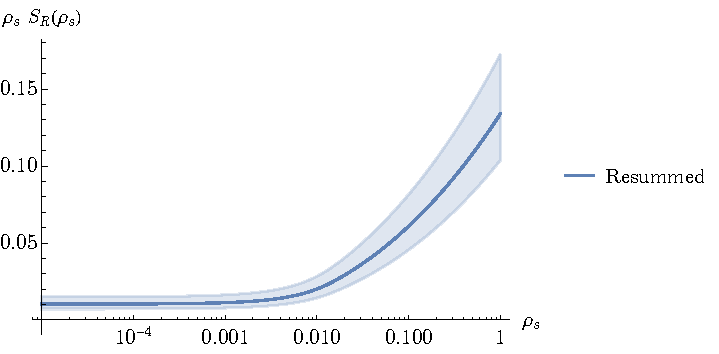
\includegraphics[width=0.9\textwidth]{figures/resummation_plot.pdf}

		\caption{\label{all-fig:resummed result}NLL resummed distribution of the soft function $S_R(\rho_s)$, from Eq.~\ref{all-eq:NLL soft function}. The top figure is the full range of $\rho_s$, while the bottom is zoomed in for small values of $\rho_s$. The running of $\alpha_s$ is fixed at the $Z$ boson mass, $\alpha_s(\SI{91.2}{\giga\electronvolt}) = 0.118$, from \cite{particle_data_group_review_2020}. The running is fixed below \SI{1}{\giga\electronvolt} in order to avoid the Landau pole at \SI{246}{\mega\electronvolt} \cite{larkoski_elementary_2019-1}. Uncertainty is estimated by varying $\mu$ within $\mu = \xi Q$ for $\xi \in [1/2, 2]$.}
	\end{center}
	\end{figure}

	On its own, the soft function $S_R$ does not have any physical meaning --- this much is clear from the manifest dependence on the arbitrary energy scale $\mu$. Physical meaning comes only in the context of the full cross section of Eq.~\ref{all-eq:full resummed result}, where we would expect to find (and, in fact, we would require) that all $\mu$-dependence cancel.\footnote{This cancellation is a strong cross-check to determine whether we have performed the calculation correctly.} Unfortunately, this means that until the entire distribution has been calculated, there is little we can do to satisfactorily convince ourselves that Eq.~\ref{all-eq:resummed inverse Laplace transform} is correct. The fact that Fig.~\ref{all-fig:resummed result} looks reasonable (i.e., it is smooth and continuous, the uncertainty is not massive, and $\rho_s S_R(\rho_s)$ does not blow up as $\rho_s \to 0$) is, however, a good start.


% \ifstandalone
% \bibliographystyle{../bsts/JHEP} 
% \bibliography{../jet_substructure}
% \fi
\end{document}
